\chapter{گزارش}

\section{مسئله}
	
در این پروژه قصد داشتیم تا پارامترهای مدل کانال در
\lr{Large-scale}
 را در یک سامانه مخابرات بی‌سیم تخمین بزنیم. 

در مدل یک کانال محوشدگی از دیدگاه 
\lr{Large-scale}، 
دو عامل افت مسیر و سایه‌شدگی نقش اساسی را ایفا می‌کردند. می‌دانیم که کانال را در حضور این دو عامل میتوان به صورت زیر مدل نمود:
\begin{figure}[H]
	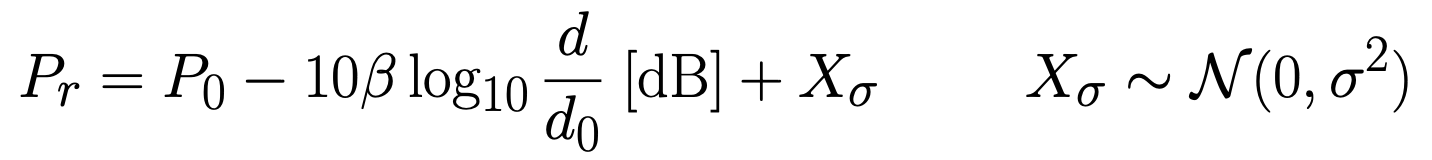
\includegraphics[width=0.75\columnwidth]{Picture/formula.png}
	\centering
\end{figure}
در این پروژه نیز تلاش شد راه حلی ارائه شود تا این این دو عامل تخمین زده شوند.

ما در این پروژه با داده‌های تست درایو در یک شبکه سلولی مواجه بودیم که شامل قدرت سیگنال دریافتی (به همراه موقعیت جغرافیایی هر اندازه‌گیری) بود. هدف ما این بود که پارامترهای مربوط به مدل افت مسیر، شامل قدرت فرستاده شده (Pt)، ضریب افت مسیر (n)، و واریانس نویز گاوسی (σ²) را تخمین بزنیم.
	
\section{راه حل}

ابتدا نرم‌افزاری در بستر اندروید پیاده‌سازی کردیم که از طریق آن توان دریافتی تلفن همراه و اطلاعات موقعیت مکانی آن را جمع‌آوری کند و پایگاه داده‌ای از این اطلاعات جمع آوری کردیم.

سپس به سراغ تخمین پارامترهای مجهول در فرمول رفتیم. ما با یک معادله‌ی خطی رو به رو بودیم که 
\lr{P\textsubscript{r}}
همان 
\lr{Y}،
\lr{10log\textsubscript{10}(d / d\textsubscript{0})}
همان
\lr{X}،
\lr{$\beta$}
همان شیب خط
و 
\lr{P\textsubscript{0}}
هم عرض از مبدا آن بود.

برای حل این مسئله، ما از روش رگرسیون خطی استفاده کردیم تا بهترین خطی که بر داده‌هایی که جمع‌آوری شده، متناسب می‌شود را پیدا کنیم و متغیرهایمان را از این خط استخراج کنیم.

برای پیدا کردن 
\lr{$\sigma$}
نویز هم از اختلاف خط به دست آمده از رگرسیون خطی و خط به دست آمده از جمع‌آوری داده‌ها استفاده کردیم.

\section{توضیح کد}
	
کد پروژه از ۲ بخش تشکیل شده است. نرم‌افزار اندرویدی با زبان کاتلین توسعه داده‌ شده و پیدا کردن متغیرها در زبان پایتون پیاده‌سازی شده است. 

قسمت پایتونی از ماژول‌های مختلفی تشکیل شده است که به پیوست این گزارش ارسال شده‌اند. در اینجا فقط به بخش اصلی آن می‌پردازیم.	

\begin{lstlisting}[language=Python]
// main.py
from db.utils import get_connection
from data.read import read_data
import numpy as np
from scipy import stats
from utils.distance import haversine
import pandas as pd

def prepare_data() -> pd.DataFrame:
	conn = get_connection("exported_database.sql")
	df = read_data(conn)
	return df

def calc_distances(df: pd.DataFrame):
	base_station_loc = df.iloc[0][['latitude', 'longitude']]
	df['distance'] = df.apply(lambda row: haversine(base_station_loc['latitude'], base_station_loc['longitude'], row['latitude'], row['longitude']), axis=1)

if __name__ == "__main__":
	df = prepare_data()
	calc_distances(df)
	
	df = df[df['distance'] > 0.0]
	
	# Pr = P0 - 10 * beta * log10(d/d0) + sigma²
	
	Pr = df['rsrp'].to_numpy()
	d = df['distance'].to_numpy()
	
	d0 = 1.0  # Reference distance (d0) in km, to match the unit of our calculated distances
	X = 10 * np.log10(d / d0)
	
	# Perform linear regression
	slope, intercept, _, _, _ = stats.linregress(X, Pr)
	
	beta_estimate = -slope
	P0_estimate = intercept
	
	# Estimate the noise standard deviation (sigma) by calculating the residuals
	residuals = Pr - (P0_estimate - beta_estimate * X)
	sigma_squared_estimate = np.var(residuals)
	sigma_estimate = np.sqrt(sigma_squared_estimate)
	
	print("Estimated Parameters:\n")
	print("Power (P0): {:.2f} dBm".format(P0_estimate))
	print("Path Loss Exponent (beta): {:.2f}".format(beta_estimate))
	print("Gaussian Noise Standard Deviation: {:.2f}".format(sigma_estimate))
	
\end{lstlisting}

همان‌طور که در این قطعه کد مشاهده می‌شود، با استفاده از رگرسیون خطی، شیب و عرض از مبدا این خط به دست می‌آید که یعنی ۲ تا از متغیرهای مجهول ما یعنی 
\lr{$\beta$}
و
\lr{P\textsubscript{0}}
از این طریق به دست آمده اند. 

پارامتر آخر یعنی انحراف استاندارد نویز هم از اختلاف خط به دست آمده از رگرسیون خطی و خط به دست آمده از داده‌های جمع‌آوری شده، به دست آمده است.
